\documentclass[a4paper,12pt]{report}
\usepackage[font=small,labelfont=bf]{caption} 
\usepackage[headheight=150pt]{geometry}
\usepackage[square,numbers]{natbib}
\usepackage[portuguese]{babel}
\usepackage[nottoc]{tocbibind}
\usepackage[utf8]{inputenc}
\usepackage[T1]{fontenc}
\usepackage{amsmath}
\usepackage{caption}
\usepackage{enumitem}
\usepackage{fancyhdr}
\usepackage{float}
\usepackage{graphicx}
\usepackage{hyperref}
\usepackage{imakeidx}
\usepackage{listings}
\usepackage{indentfirst} 
\usepackage{lipsum}
\usepackage{pdfpages}
\usepackage{subcaption}
\usepackage{tikz}
\usepackage{color}
\usepackage{listings}

\definecolor{dkgreen}{rgb}{0,0.6,0}
\definecolor{gray}{rgb}{0.5,0.5,0.5}
\definecolor{mauve}{rgb}{0.58,0,0.82}
\lstset{ 
  language=Java,
  basicstyle=\footnotesize,
  numbers=left,
  numberstyle=\tiny\color{gray},
  stepnumber=1,
  numbersep=5pt,
  backgroundcolor=\color{white},
  showspaces=false,
  showstringspaces=false,
  showtabs=false,
  frame=single,
  rulecolor=\color{black},
  tabsize=4,
  captionpos=b,
  breaklines=true,
  breakatwhitespace=false,
  title=\lstname,
  keywordstyle=\color{blue},
  commentstyle=\color{dkgreen},
  stringstyle=\color{mauve},
  escapeinside={\%*}{*)},
  morekeywords={*,...}
}

\linespread{1.2}
\setlist[itemize]{noitemsep, topsep=0pt}
\pagestyle{fancy}
\bibliographystyle{unsrtnat}
\usetikzlibrary{shapes,arrows, snakes}
\tikzstyle{startstop} = [rectangle, rounded corners, minimum width=2cm, minimum height=1cm,text centered, draw=black]
\tikzstyle{startstop} = [rectangle, rounded corners, minimum width=2cm, minimum height=1cm,text centered, draw=black]
\tikzstyle{process} = [rectangle, minimum width=2cm, text width=6cm,minimum height=1cm, text centered, draw=black]
\tikzstyle{decision} = [diamond, minimum width=2cm, minimum height=1cm, text centered, draw=black]
\tikzstyle{io} =[trapezium, trapezium left angle=70, trapezium right angle=110, minimum height=1cm, text centered, draw=black]
\tikzstyle{arrow} = [thick,->,>=stealth]

\lhead{
\includegraphics[width=2cm]{img/ua.png}}
\rhead{Cláudio Henriques}
\title{
    \protect
\includegraphics[scale=0.8]{img/ua.png}\\
    [4cm]Trabalho 1\\
    Seminário de Matemática Aplicada
}

\author{
    Cláudio Henriques\\
    Mestrado em Matemática e Aplicações
}

\makeindex

\begin{document}

\maketitle
\tableofcontents
\listoffigures

\chapter{Introdução}

No presente relatório é apresentado o algoritmo desenvolvido para a coloração dos vértices de um determinado grafo, utilizando a sua matriz de adjacência para definir uma estrutura abstracta para o representar. É ainda apresentado um algoritmo de pesquisa em profundidade.

Estes algoritmos foram implementados recorrendo à linguagem de programação \textit{Java}. Foi ainda desenvolvido um pequeno script em \textit{R} para a visualização do grafo aplicando as colorações obtidas nos algoritmos.

\section{\textit{Java}}

A escolha da linguagem baseou-se essencialmente pelos recursos que esta oferece. Apesar de não ser tão rápida e consumir mais recursos computacionais quando comparada com o \textit{Python} ou \textit{Julia}, o \textit{Java} oferece um bom suporte para o desenvolvimento de algoritmos sob o velho conhecido paradigma \textit{Object-oriented programming (OOP)} (em português: Programação Orientada a Objetos (POO)).

A opção de implementar o trabalho em torno deste paradigma permite desenvolver \textit{módulos} que possam ser usados futuramente noutros trabalhos relacionados com esta temática. Um exemplo simples é poder usar a estrutura de dados abstrata criada para representar um grafo num outro trabalho/projeto em que seja necessário esta estrutura para desenvolver outro tipo de algoritmos. Assim permite a diminuição de código redundante (i.e. implementar várias vezes a mesma estrutura da dados sempre que necessitar de a utilizar em ambientes diferentes).

\section{Estruturas de Dados}

As estrturuas de dados desenvolvidas ao longo do trabalho são:
\begin{itemize}
    \item \textbf{Grafo} (\textit{Graph.java}): representar um objeto do tipo grafo (recorrendo à sua matriz de adjacência);
    \item \textbf{Vértice} (\textit{Vertex.java}):
    A estrutura anterior instância uma estrutura auxiliar para representar cada vértice como um objeto único. Desta forma um grafo é representado com um conjunto de vértices.
    (Lógicamente seria óbvio representar um grafo como um conjunto de vértices e arestas, contudo as arestas (neste caso) não são estritamente necessárias ao desenvolvimento dos algoritmos, recorrendo apenas a atributos no objeto vértice para identificar os seus \textit{vizinhos})
\end{itemize}

\section{Algoritmos}

\begin{itemize}
    \item \textbf{Coloração dos vértices, versão 1} (\textit{ColorizeVersion1.java}):
    Implementa o algoritmo apresentado nas aulas para a coloração dos vértices de um grafo, recorrendo à sua matriz de adjacência.
    \item \textbf{Coloração dos vértices, versão 2} (\textit{ColorizeVersion2.java}):
    Implementadado como uma extensão da versão 1 deste algoritmo, altera apenas a ordem pela qual percorre os vértices do grafo.
    \item \textbf{Coloração dos vértices, versão 3} (\textit{ColorizeVersion3.java}): Organiza os vértices pela ordem de maior grau, sendo este o critério para os percorrer e atribuir uma cor.
    \item \textbf{\textit{Depth First Search} (DFS)} (\textit{DFS.java}):
\end{itemize}

\section{Módulos extra}

\begin{itemize}
    \item \textbf{Ficheiro de logs} \textit{(WriteLogFile.java)}
    Para auxiliar na descrição dos algoritmos foi criado um sistema de \textit{logs}, isto é, quando o algoritmos efetua alguma operação, esta é registada num ficheiro do tipo \textit{*.txt}, detalhando cada passo, por ordem cronológica.
    
\end{itemize}

%\section{Code examples}

%\lstinputlisting[language=Java]{Graph.java}

\chapter{Implementação}

Nesta secção é apresentado e explicado a implementação das estruturas de dados que foram desenvolvidas por forma a tornar os algoritmos mais eficientes.

Algumas linhas de código foram omitidas para simplificar a explicação, por exemplo, a implementação da criação do ficheiro auxiliar com a matriz de adjacência que vai ser lida pelo script \textit{R} uma vez que este processo não é essencial para o desenvolvimento dos algoritmos.
Foram também omitidas as linhas correspondentes à implementação dos ficheiros de \textit{log}.

Todo o código está comentado e pode ser visto em  \href{https://github.com/cfchenr/sma}{aqui}

\section{Grafo (\textit{Graph.java})}

Esta estrutura abstracta usa um \textit{ArrayList} para representar o conjunto de vértices pertencentes ao objeto (vertexList).

Cada grafo é identificado por um \textit{id} e contém um atributo chamado \textit{order} que representa a ordem do grafo.

\begin{lstlisting}[language=Java]
    private String id;
    private int order;
    private ArrayList<Vertex> vertexList;
\end{lstlisting}

Neste caso o \textit{id} é o nome do ficheiro com a matriz de adjacência que é lida. Por exemplo, se construir um grafo recorrendo à matriz de adjacência do ficheiro \textit{A.txt}, o \textit{id} deste grafo é definido como A.

\begin{lstlisting}
    id = file.split("/")[1].split("\\.")[0];
\end{lstlisting}

À medida que cada linha do ficheiro com a matriz de adjacência é lida é adicinado à lista de vértices um novo vértice (pois cada linha da matriz identifica um vértice do grafo). Estes são identificados por um número que é igual à ordem do grafo na iteração anterior.

Por exemplo, se ainda não foram lidas nenhuma linha então o primeiro vértice que é criado é representado por 0. Na linha seguinte é criado um novo vértice, desta vez já é representado pelo número 1.

Consequentemente a ordem do grafo é o número de linhas da matriz de adjacência.

\begin{lstlisting}
    while (scf.hasNextLine()) {
        vertexList.add(new Vertex(order));       
        order++;
    }
\end{lstlisting}

Seguidamente são lidos cada uma das entradas de cada linha da matriz para se definir as vizinhanças de cada vértice. Desta forma, a cada entrada da linha que é lida, se for $1$ ou $-1$ então significa que o vértice que é representado pelo índice da linha da matriz é vizinho do vértice representado pelo índice da coluna da entrada em questão.

Consequentemente, se for $1$ então definimos que o vértice representado pelo índice da linha da matriz é sucessor do vértice representado pelo índice da coluna da entrada em questão. Lógicamente também definimos que o índice da coluna da entrada em questão é predecessor do vértice representado pelo índice da linha da matriz. (A distinção entre sucessor e predecessor é implementada na estrutura \textit{Vertex.java}, através da distinção do segundo argumento que é passado na função. Esta anotação é explicanda mais à frente na secção \ref{vertex}).

Analogamente utilizamos a mesma metodologia no caso da entrada ser $-1$.

\begin{lstlisting}
    for (int k = 0; k < line.length; k++) {
        if (line[k].equals("1")) {
            vertexList.get(j).setNeighbors(k, 1);
            vertexList.get(k).setNeighbors(j, -1);
        } else if (line[k].equals("-1")) {
            vertexList.get(j).setNeighbors(k, -1);
            vertexList.get(k).setNeighbors(j, 1);
        }
    }
\end{lstlisting}

O método \textit{getId ()} retorna o \textit{id} deste grafo.

\begin{lstlisting}
        return id;
\end{lstlisting}

O método \textit{getOrder ()} retorna a ordem do grafo.

\begin{lstlisting}
        return order;
\end{lstlisting}

O método \textit{getVertexList ()} retorna a lista com todos os vértices do grafo.

\begin{lstlisting}
        return vertexList;
\end{lstlisting}

O método \textit{isNeighbor (int k, int y)} retorna um valor \textit{booleano} para dar resposta à pergunta "k é vizinho de y?". Reparemos que k ser vizinho de y é a mesma coisa que y ser vizinho de k.

\begin{lstlisting}
        return (vertexList.get(k).isNeighbor(y) || vertexList.get(y).isNeighbor(k));
\end{lstlisting}


O método \textit{getVertexByDegree ()} retorna uma lista de vértices por ordem crescente do grau do vértice.

Neste método é criada uma estrutura temporária para armazenar os vértices pela ordem pretendida.

Num primeiro momento, é obtido o grau máximo de todos os vértices. Após esta operação é adicionada à estrutura temporária os vértices que têm o grau igual ao grau máximo (os vértices são adicionamos sempre ao inicio da lista, o que permite criar a lista por ordem crescente de grau dos vértices). Quando não houver mais vértices com o grau máximo então é reduzido o valor máximo numa unidade voltando a efetuar o processo anterior. Este ciclo termina quando o valor máximo for 0.

Por fim é retornada a estrutura temporária, sendo esta uma lista com os vértices organizados por ordem crescente do grau.

\begin{lstlisting}
        ArrayList<Vertex> temp = new ArrayList<Vertex>();
        int max = 0;
        for (int i = 0; i < vertexList.size(); i++)
            if (vertexList.get(i).getDegree() >= max) 
                max = vertexList.get(i).getDegree();
        while (max >= 0) {
            for (int i = 0; i < vertexList.size(); i++) {
                if (vertexList.get(i).getDegree() == max){
                    temp.add(0, vertexList.get(i));
                    vertexList.remove(i);
                    i--;
                }
            }       
            max--;
        }
        return temp;
\end{lstlisting}

O método \textit{sortVertexByDegree ()} organiza a lista de vértices deste grafo pela ordem do grau de cada vértice.

\begin{lstlisting}
        vertexList = getVertexByDegree();
\end{lstlisting}

O método \textit{setDefaultColorVertexes ()} define a cor de cada vértice como 0 (cor inicial).

\begin{lstlisting}
        for (int i = 0; i < vertexList.size(); i++)
            vertexList.get(i).setColor(0);
\end{lstlisting}

\section{Vértice (\textit{Vertex.java})}\label{vertex}

Esta estrutura representa um vértice, identificado por um id, cor, ordem, por um atributo que define se o vértice foi ou não visitado, por uma lista de vértices sucessores e uma lista de predecessores.

\begin{lstlisting}
    private int id, color, order;
    private boolean visited;
    private ArrayList<Integer> successorList, predecessorList;
\end{lstlisting}

O método \textit{getId ()} retorna o \textit{id} do vértice.

\begin{lstlisting}
    return id;
\end{lstlisting}

O método \textit{setColor (int color)} define a cor do vértice com a cor color.

\begin{lstlisting}
    this.color = color;
\end{lstlisting}

O método \textit{getColor ()} retorna a cor do vértice.

\begin{lstlisting}
    return color;
\end{lstlisting}

O método \textit{setOrder (int order)} define a ordem do vértice com o número order.

\begin{lstlisting}
    this.order = order;
\end{lstlisting}

O método \textit{getOrder ()} retorna a ordem do vértice.

\begin{lstlisting}
    return order;
\end{lstlisting}

O método \textit{setVisited ()} define o vértice como visitado.

\begin{lstlisting}
    visited = true;
\end{lstlisting}

O método \textit{isVisited ()} retorna um booleano que indica se o vértice já foi ou não visitado.

\begin{lstlisting}
    return visited;
\end{lstlisting}

O método \textit{setNeighbors (int k, int ps)} define este vértice como vizinho do vértice identificado por k. Se ps for $1$ então o vértice k é sucessor, caso contrário k é predecessor.

\begin{lstlisting}
    if (ps == 1) {
        if (!successorList.contains(k))
            successorList.add(k);
    }
    else if (ps == -1) {
        if (!predecessorList.contains(k))
            predecessorList.add(k);
    }
\end{lstlisting}

O método \textit{isNeighbor (int k)} retorna um valor booleano que indica se o vértice é vizinho do vértice k.

\begin{lstlisting}
    return (successorList.contains(k) || predecessorList.contains(k));
\end{lstlisting}

O método \textit{getNeighborList ()} retorna a lista de sucessores e predecessores do vértice.

\begin{lstlisting}
    Set<Integer> set = new HashSet<Integer>();
    set.addAll(successorList);
    set.addAll(predecessorList);
    return new ArrayList<Integer>(set);
\end{lstlisting}

O método \textit{getSucessorList ()} retorna a lista de sucessores do vértice.

\begin{lstlisting}
    return sucessorList;
\end{lstlisting}

O método \textit{getPredecessorList ()} retorna a lista de predecessores do vértice.

\begin{lstlisting}
    return predecessorList;
\end{lstlisting}

O método \textit{getDegree ()} retorna o grau do vértice. Este é igual ao número de visinhos do vértice.

\begin{lstlisting}
    return getNeighborList().size();
\end{lstlisting}

\section{Coloração dos vértices, versão 1}

Esta implementação recebe um objeto do tipo grafo (\textit{Graph.java}) e contém um conjunto de métodos que permite desenvolver um algoritmo de \textit{fácil} leitura.
Quando invocada, esta implementação guarda a lista dos vértices do grafo e define todos os vértices com a cor $0$ (para garantir que o vértice não foi colorido anteriormente com outra cor distinta).

\begin{lstlisting}
    graph.setDefaultColorVertexes();
    vertexList = graph.getVertexList();
\end{lstlisting}

O método \textit{setColorVertex (int id)} define a cor do vértice identificado pelo \textit{id} com a primeira cor disponível (tendo em conta os seus vizinhos), com recurso ao método \textit{getFirstColorAvailable ()}. 
No caso do \textit{id} ser $-1$ significa que o vértice a colorir é o último vértice da lista.
Após obter o vértice correspondente ao \textit{id} obtém a primeira cor disponível (\textit{color}) e atribui ao vértice a cor color.

\begin{center}
    \begin{tikzpicture}[node distance=1.5cm]
        \node (start) [startstop] {Início};
        \node (dec1) [decision, below of=start, yshift=-0.75cm] {id = -1?};
        \node (proc1) [process, right of=dec1, xshift=4cm] {Obter o vértice identificado pelo id};
        \node (proc2) [process, below of=dec1, yshift=-0.75cm] {Obter o último vértice da lista};
        \node (proc3) [process, below of=proc2] {Obter a primeira cor disponível
        (\textit{getFirstColorAvailable()})};
        \node (proc4) [process, below of=proc3] {Colorir o vértice com a cor obtida};
        \node (stop) [startstop, below of=proc4] {Fim};
        \draw [arrow] (start) -- (dec1);
        \draw [arrow] (dec1) -- node[anchor=south] {Não} (proc1);
        \draw [arrow] (dec1) -- node[anchor=east] {Sim} (proc2);
        \draw [arrow] (proc2) -- (proc3);
        \draw [arrow] (proc1) .. controls +(down:3cm) and +(right:5cm) .. (proc3);
        \draw [arrow] (proc3) -- (proc4);
        \draw [arrow] (proc4) -- (stop);
    \end{tikzpicture}    
\end{center}

\begin{lstlisting}
    Vertex vertex;
    if (id == -1)   
        vertex = vertexList.get(vertexList.size()-1);
    else
        vertex = vertexList.get(id);
    int color = getFirstColorAvailable();
    vertex.setColor(color);
\end{lstlisting}

O método \textit{getFirstColorAvailable ()} analisa uma fila de cores e retorna a cor mínima disponível. Esta fila é preenchida no método \textit{saveNeighborColors (int j)}.
Inicialmente começa com a cor mínima k = 1 e verifica se esta cor existe na lista de cores. 
No caso de exisitir então k passa a ser igual a 2 e volta a verificar se 2 existe na lista de cores. Este processo é repetido até encontrar um k que não conste na lista de cores.

\begin{center}
    \begin{tikzpicture}[node distance=1.5cm]
        \node (start) [startstop] {Início};
        \node (proc1) [process, below of=start] {k=1};
        \node (dec1) [decision, below of=proc1, yshift=-0.75cm] {\tiny Lista contém k?};
        \node (proc2) [process, right of=dec1, xshift=4cm] {Devolve k};
        \node (proc3) [process, below of=dec1, yshift=-1cm] {k++};
        \node (stop) [startstop, below of=proc3] {Fim};
        \draw [arrow] (start) -- (proc1);
        \draw [arrow] (proc1) -- (dec1);
        \draw [arrow] (dec1) -- node[anchor=south] {Não} (proc2);
        \draw [arrow] (dec1) -- node[anchor=east] {Sim} (proc3);
        \draw [arrow] (proc3) .. controls +(left:5cm) and +(left:5cm) .. (dec1);
        \draw [arrow] (proc2) .. controls +(down:3cm) and +(right:3cm) .. (stop);        
    \end{tikzpicture}    
\end{center}

\begin{lstlisting}
    int k = 1;
    while(colors.contains(k))
        k++;
    return k;
\end{lstlisting}

O método \textit{saveNeighborColors (int j)} guarda as cores dos vizinhos do vértice identificado por j. 
Nesta implementação, apenas verifica se os vértices anteriores são vizinhos, uma vez que como a ordem pela qual são percorridos os vértices começa no primeiro vértice até ao último, então aquando do vértice j ainda só foram coloridos os vértices anteriores.
Quando encontrar um vértice vizinho, adiciona a cor deste à lista de cores.

\begin{center}
    \begin{tikzpicture}[node distance=1.5cm]
        \node (start) [startstop] {Início};
        \node (for1) [io, below of=start] {Percorrer a lista de vértices (i) até j};
        \node (dec1) [decision, below of=for1, yshift=-0.75cm] {\tiny j vizinho de i?};
        \node (proc1) [process, below of=dec1, yshift=-0.75cm] {Adiciona a cor do vértice i à lista de cores};
        \node (stop) [startstop, below of=proc1] {Fim};
        \draw [arrow] (start) -- (for1);
        \draw [arrow] (for1) -- (dec1);
        \draw [arrow] (dec1) -- node[anchor=east] {Sim} (proc1);
        \draw [arrow] (dec1) .. controls +(left:5cm) and +(left:7.5cm) .. node[anchor=north] {Não} (for1);
        \draw [arrow] (for1) .. controls +(right:8cm) and +(right:8cm) ..(stop);
        \draw [arrow] (proc1) .. controls +(left:8cm) and +(left:8cm) .. (for1);
    \end{tikzpicture}    
\end{center}

\begin{lstlisting}
    colors = new LinkedList<Integer>();
    for (int i = 0; i < j; i++)
        if (vertexList.get(j).isNeighbor(vertexList.get(i).getId()))
            colors.add(vertexList.get(i).getColor());
\end{lstlisting}

O método \textit{getVertexList ()} retorna a lista dos vértices do grafo.

\begin{lstlisting}
    return vertexList;
\end{lstlisting}

\subsection{Algoritmo}

Em suma, seja v1 um objeto do tipo \textit{ColorizeVersion1.java}, definimos a cor do vértice 0 (o primeiro vértice do grafo) com a primeira cor disponível (como é o primeiro vértice, a cor atribuida a este será 1).
Após este processo, percorre-se todos os restantes vértices. A cada um destes, guarda-se a cor dos vértices anteriores que são seus vizinhos e seguidamente é definida a cor do vértice j com a cor mínima disponível (tendo em conta as cores obtidas no processo anterior).
O algoritmo final terá o seguinda aspeto:
\begin{lstlisting}
    v1.setColorVertex(0);
    for (int j = 1; j < v1.getVertexList().size(); j++) {
        v1.saveNeighborColors(j);
        v1.setColorVertex(j);
    }
\end{lstlisting}

\section{Coloração dos vértices, versão 2}

Esta implementação, sendo uma extensão da anterior, é em grande parte igual à versão 1. A alteração que implementa é a ordem pela qual verifica os vértices vizinhos, ou seja, apenas verifica os vértices desde o fim até ao vértice j.

\begin{lstlisting}
    colors = new LinkedList<Integer>();
    for (int i = vertexList.size()-1; i > j; i--)
        if (vertexList.get(j).isNeighbor(vertexList.get(i).getId()))
            colors.add(vertexList.get(i).getColor());
\end{lstlisting}

\subsection{Algoritmo}

Em suma, seja v2 um objeto do tipo \textit{ColorizeVersion2.java}, definimos a cor do último vértice com a primeira cor disponível (como é o primeiro vértice, a cor atribuida a este será 1).
Após este processo, percorre-se todos os restantes vértices, começando pelo fim (contráriamente à versão anterior). A cada um destes, guarda-se a cor dos seus vizinhos e seguidamente é definida a cor do vértice j com a cor mínima disponível (tendo em conta as cores dos seus vizinhos).
O algoritmo final terá o seguinda aspeto:

\begin{lstlisting}
    for (int j = v2.getVertexList().size()-2; j >= 0; j--) {
        v2.saveNeighborColors(j);
        v2.setColorVertex(j);
    }
\end{lstlisting}

\section{Coloração dos vértices, versão 3}

Esta implementação, quando invocada, tem o mesmo comportamento da versão 1 e 2, contudo organiza os vértices pela ordem do seu grau. Uma outra diferença nesta implementação é que ao invês de usar uma lista de cores usa um dicionário em que a chave é o código da cor e o valor é 1 (0 no caso da cor fazer parte da coloração dos vértices vizinhos de um determinado vértice, e neste caso não é adicionado ao dicionário de cores, 1 no caso de algum vizinho ter a cor identificada pelo código da cor).

\begin{lstlisting}
    colors = new Hashtable<Integer, Integer>();
    vertexByDegree = graph.getVertexByDegree();
\end{lstlisting}

No método \textit{setColorVertex (int id)}, ao invés de se obter os vértices a partir da lista de vértices, o algoritmo recorre à lista dos vértices ordenados por grau. O restante código é igual ao implementado nas versões anteriores.

\begin{lstlisting}
    Vertex vertex;
    if (id == -1)   
        vertex = vertexList.get(vertexByDegree.get(vertexByDegree.size()-1).getId());
    else
        vertex = vertexList.get(vertexByDegree.get(id).getId());
    int color = getFirstColorAvailable();
    vertex.setColor(color);
\end{lstlisting}

O método \textit{saveNeighborColors (int j)} tira proveito do facto de cada vértice ter associado uma lista de vértices vizinhos. Isto permite que o algoritmo não tenha de percorrer todos os vértices do grafo e verificar se algum é vizinho do vértice j e nesse caso adicionar a sua cor à tabela de cores. Neste caso, o algoritmo percorre apenas os vértices que fazem parte da lista de vizinhos do vértice j e adiciona a sua cor à tabela de cores.
Contráriamente a uma lista, a tabela (sendo ela um dicionário) caso contenha a cor que está a adicionar simplesmente atualiza o seu valor (que neste caso fica exatamente igual). Por exemplo, considera-se uma tabela de cores que já contem a cor 2 e 5. Então os valores associados a 2 e 5 é 1 (como foi explicado em cima). Quando se adiciona novamente a cor 2 ou a cor 5, ao invés de criar uma nova entrada nesta tabela de cores, simplesmente verifica se ela já existe antes de criar.

\begin{lstlisting}
    colors = new Hashtable<Integer, Integer>();   
    for (int i = 0; i < vertexList.get(vertexByDegree.get(j).getId()).getNeighborList().size(); i++)
        colors.put(vertexList.get(vertexList.get(vertexByDegree.get(j).getId()).getNeighborList().get(i)).getColor(), 1);
\end{lstlisting}

\subsection{Algoritmo}

Em suma, a implementação deste algoritmo segue a mesma lógica da versão 2, pois uma vez que os vértices estão ordenados por ordem crescente de grau, então começa a percorrer do fim para o início, por forma a atribuir primeiramente as cores aos vértices com maior grau.
Seja v3 um objeto do tipo \textit{ColorizeVersion3.java}:

\begin{lstlisting}
    for (int j = v3.getVertexList().size()-2; j >= 0; j--) {
        v3.saveNeighborColors(j);
        v3.setColorVertex(j);
    }
\end{lstlisting}

\section{\textit{Depth First Search} (DFS)}

\subsection{Algoritmo}

\chapter{Exercício 1}

\section{Análise e Resultados}

Seja $I$ a matriz 
$\begin{bmatrix}
    0&1&0&1&0&1\\
    1&0&1&0&0&1\\
    0&1&0&0&1&0\\
    1&0&0&0&1&0\\
    0&0&1&1&0&1\\
    1&1&0&0&1&0
\end{bmatrix}$ e seja $graph$ um objeto do tipo \textit{Graph.java} construido com recurso à matriz $I$.

Implementamos o objeto $ColorizeVersion1.java$ usando o grafo $graph$.
A coloração obtida é a representada no seguinte grafo:

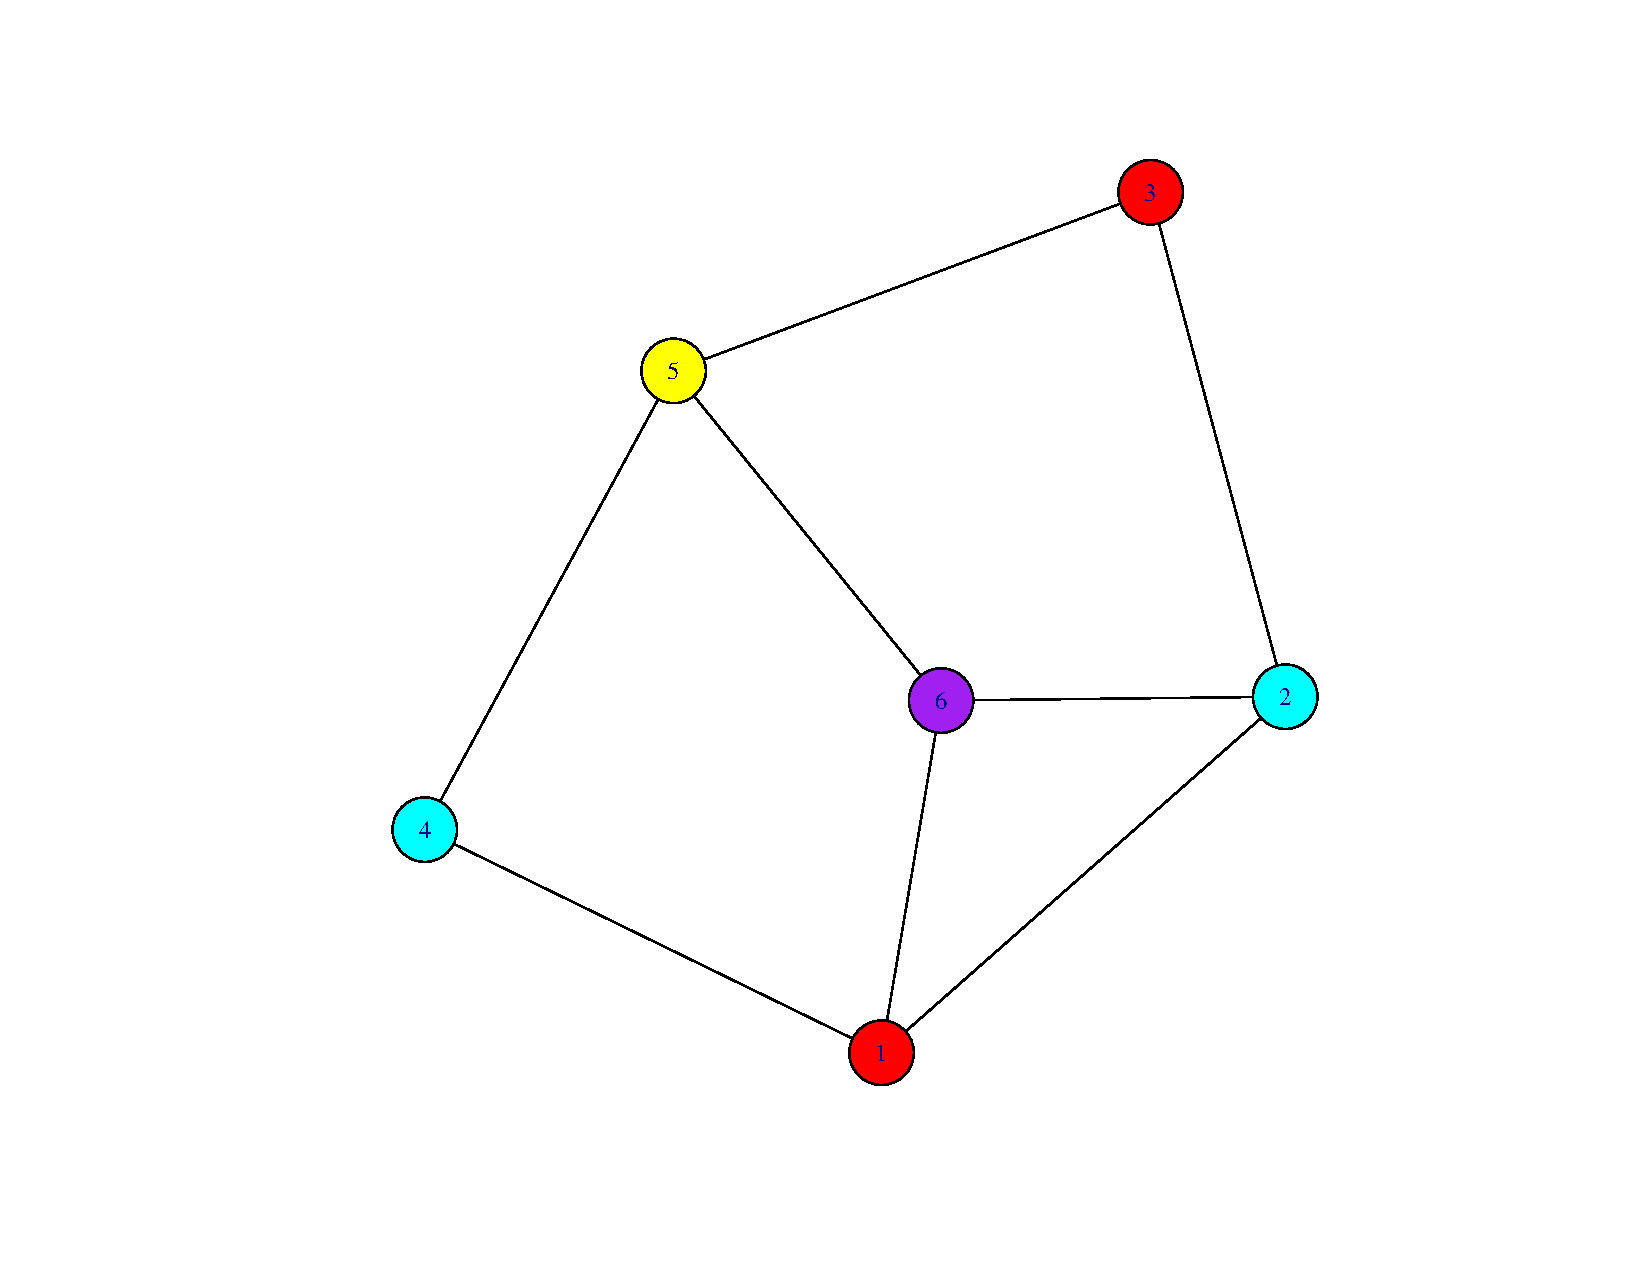
\includepdf[pages=-, scale=0.5]{v1I.pdf}

Seja $F$ a matriz 
$\begin{bmatrix}
    0&1&1&1&1&0&1&1&1&1\\
    1&0&1&1&1&0&0&1&0&1\\
    1&1&0&1&1&1&1&1&1&1\\
    1&1&1&0&1&1&0&0&1&1\\
    1&1&1&1&0&1&1&0&0&0\\
    0&0&1&1&1&0&1&1&1&0\\
    1&0&1&0&1&1&0&1&0&1\\
    1&1&1&0&0&1&1&0&1&1\\
    1&0&1&1&0&1&0&1&0&1\\
    1&1&1&1&0&0&1&1&1&0
\end{bmatrix}$ e seja $graph$ um objeto do tipo \textit{Graph.java} construido com recurso à matriz $F$.

Implementamos o objeto $ColorizeVersion1.java$ usando o grafo $graph$.
A coloração obtida é a representada no seguinte grafo:

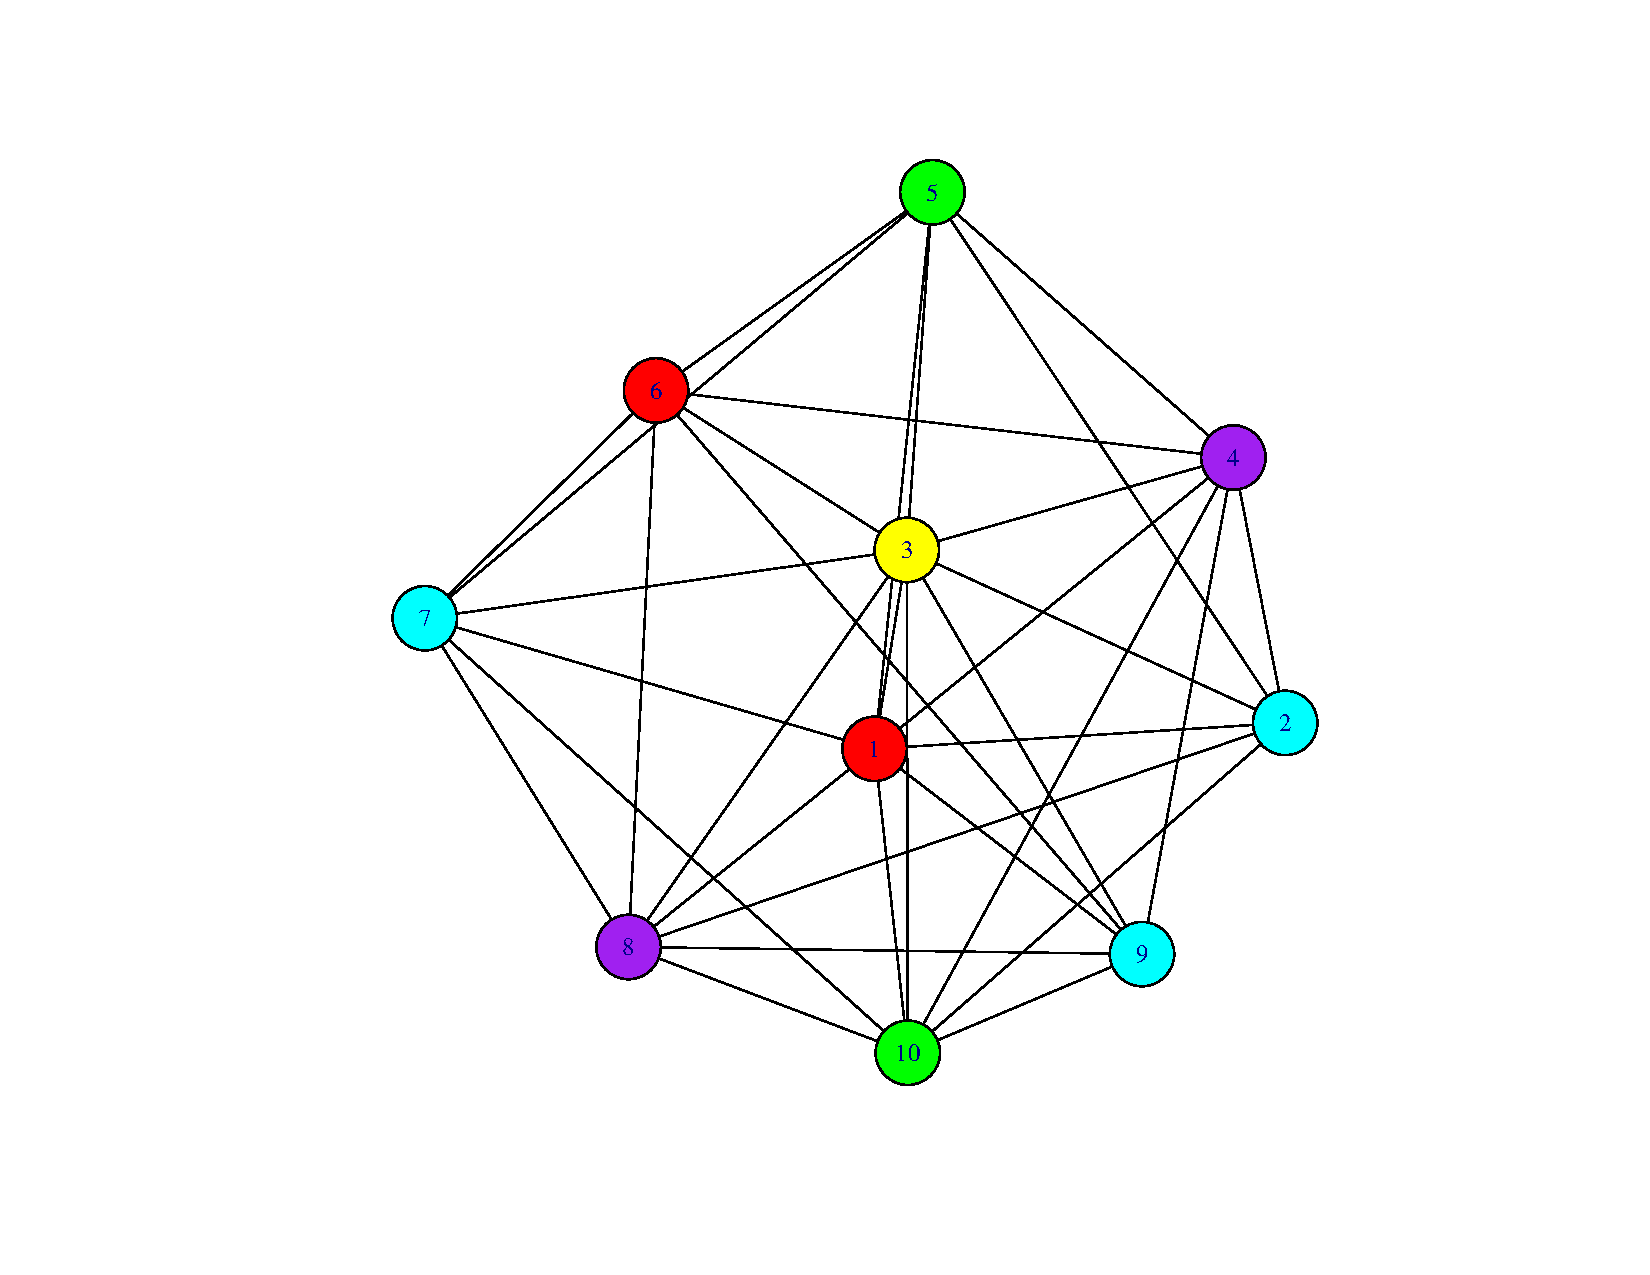
\includepdf[pages=-, scale=0.5]{v1F.pdf}

\chapter{Exercício 2}

\section{Análise e Resultados}

\chapter{Exercício 3}

\section{Análise e Resultados}

\chapter{Conclusão}

\section{Considerações futuras}

\end{document}
